\section{Structures de données}
	
Certaines des structures de données ne sont utilisées que par certains modules du programme. Il n'est donc pas nécessaire de les abstraire. En revanche, certaines de ces structures sont utilisées par plusieurs modules, c'est le cas de la liste chaînée.
	\subsection{Structures simples}
    
	\subsubsection{La structure map}
    La structure map est construite par le parseur de cartes, contenu dans le module de parsing.
	les champs de cette structure sont :
	\begin{itemize}
		\item Un entier hauteur
		\item Un entier largeur
		\item Un tableau de caractères
		\item Une structure position pour repérer le point de départ
		\item Un entier pour le maximum de checkpoints
	\end{itemize}	
    
	\subsubsection{La structure steps}
	La structure steps est un ensemble de coups relatifs à une carte. Elle est générée par le parseur de coups. Elle peut être utilisée,par exemple, pour de comparer les performences d'autres intelligences artificelles.\\
Elle contient : 
	\begin{itemize}
		\item Un entier pour le nombre d'accélérations
		\item Un entier pour le nombre d'étapes
		\item Une structure point pour la position de départ
		\item Deux tableaux de structures point contenant les positions et vitesses correspondantes
	\end{itemize}	
	\subsubsection{La structure point}
    Cette structure est exclusivement utilisée par les modules de moteur de jeu, ainsi que l'affichage graphique. \\
	La structure point est une structure simple à deux champs entiers. Ces deux nombres représentent une position sur la grille. Le moteur de jeu utilise cette structure pour communiquer une position à l'interface.\\
	
	\subsubsection{La structure node}
    La structure node est utilisée par le module de résolution d'une carte. Elle contient quatre champs entiers, correspondants à une position et une vitesse. Elle contient de plus un champs pointeur sur le noeud précédent.\\

Grâce à l'abscence de typage des données dans la liste chaînée (pointeur void), nous pouvons stocker des données de n'importe quel type dans une liste chaînée, notemment les structures point (pour le moteur de jeu) et node (pour le solveur).



	\subsection{Structures abstraites}	
    La seule structure ayant été sujet d'une abstraction est la liste chaînée.
	\subsubsection{Mise en oeuvre}
	Le type de données utilisée içi est une liste doublement chainée	
	\begin{figure}[h]
	\centering
	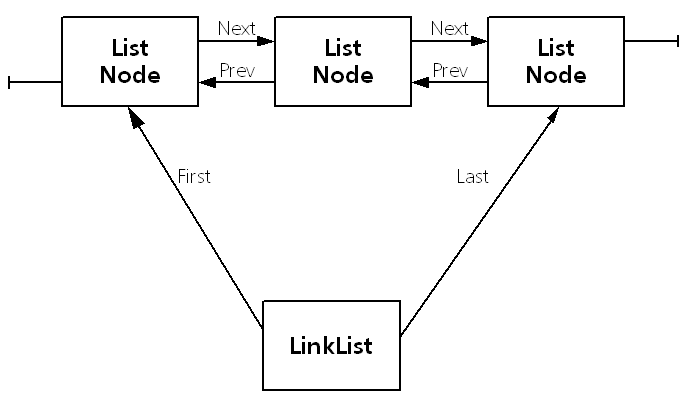
\includegraphics[scale = 0.3]{linklist.png}
    \caption{Double linked list}
    \end{figure} \\
    Les structures sont donc: \\
	\texttt{liste}
	\begin{itemize}
	\item pointeur sur l'élément tête
	\item pointeur sur l'élément queue
	\item entier nombre d'éléments (à 0 initialement)
	\end{itemize}
	\texttt{element}
    \begin{itemize}
	\item pointeur sans type sur une donnée
	\item pointeur élément sur l'élément précédent
	\item pointeur élément sur l'élément suivant
	\end{itemize}
	\subsubsection{Primitives}
  	Les primitives utilisées pour gérer la liste sont les suivantes : \\
	\texttt{list\_empty} qui teste si la liste est vide. \\
    \texttt{list\_head} renvoie la tête de la liste.\\
	\texttt{list\_tail} renvoie la queue de la liste. \\
    Celles relatives aux éléments sont :
	\texttt{list\_data} qui renvoie un pointeur sans type sur le champ donné de l'élément passé en paramètre.\\	
	\texttt{list\_next} renvoie le pointeur sur l'élément suivant. \\
	\texttt{list\_previous} renvoie le pointeur sur l'élément précédent. \\

	\subsubsection{Intérêt}
	L'abstraction de la liste chainée et de ses élements la rend utilisable par n'importe module sans qu'il n'ai connaissance de son implémentation. Cela permet notemmment de l'utiliser pour lister des coups jouables avec le solveur, ou de générer une liste de positions jouées. \\

	Le double chaînage permet de réduire la complexité de la fonction \texttt{list\_add} (qui effectue un ajout en queue). Avec une liste simple elle aurait été $\theta(n)$ en la taille de la liste, içi elle est en $\theta(1)$. De même pour la fonction de retrait en queue.\\






































